\begin{frame}
\frametitle{Outline} 
\tableofcontents
\end{frame}

%% ----------------------------------------------------------
%%  SLIDE 2 — Why static typing for dynamic languages?
%% ----------------------------------------------------------
\begin{frame}
\frametitle{Why static typing for dynamic languages?}

\vspace{-3mm}
\small
\begin{block}{Static types for dynamic languages}\setlength{\leftmargini}{1.2em}
  \begin{itemize}\setlength{\itemsep}{3pt}
    \item \textbf{Catch bugs early} and enable \textbf{tooling}: completion,
          navigation, safe refactoring
    \item \textbf{Checked documentation}: types state what functions expect and
          return; crucial when code is written by AI and read by programmers
    \item \textbf{Existing solutions fall short}: TypeScript, Flow, Hack are
          language-specific and unsound; rewriting in a typed language takes years
    \item \textbf{Needed}: a type system that is \textbf{sound},
          \textbf{gradual}, \textbf{automated}, and \textbf{open}
  \end{itemize}
\end{block}
\setbeamercolor{block body alerted}{bg=red!8}
\begin{alertblock}{Regulatory compliance}\setlength{\baselineskip}{0.85\baselineskip}
  EU and US regulations increasingly \textbf{require evidence of
  software assurance} (CRA, NIST guidelines, \ldots). A
  \emph{sound} type system is a mechanically verifiable step in that direction,
  also for AI-generated code.
\end{alertblock}

\textbf{\color{darkslateblue}The challenge: dynamic code relies on idioms that classic
type systems cannot describe}

\end{frame}

\subsection{Branching, overloading, and pattern matching}

% language tag in the top right corner of TypeScript code boxes (put at the end of the first line)
\newcommand{\tsLabel}{\hfill\textcolor{gray}{\sffamily{\scriptsize T}{\tiny YPE}{\scriptsize S}{\tiny CRIPT}}}% faked small caps: the sans font (Carlito) has none
\begin{frame}[fragile]\transdissolve
\frametitle{1. Branching and discriminated unions}\vspace{-4mm}
\begin{minted}[fontsize=\normalsize]{typescript}
type Status = "success" | "error";!\tsLabel!
function report(s: Status): number | string {
  if (s === "success") return 200;
  return "failed";
}
\end{minted}
{\small\color{gray}The result is \texttt{number} or \texttt{string} depending on the branch\par}
\pause
\vspace{-2mm}
\begin{minted}[fontsize=\normalsize]{typescript}
type Payment = !\tsLabel!
  | { kind: "card";   cardNo: string }
  | { kind: "paypal"; email: string };
\end{minted}
\vspace{-1mm}%
{\small\color{gray}A \emph{discriminated union}: the field \texttt{kind} tells which variant a payment is\par}
\pause
\begin{exampleblock}{$\Rightarrow$ Union and singleton types are needed}
\pb{"success"}, \pb{"error"}, \pb{"card"}: types with one value;\quad \pb{Status}, \pb{Payment}: their unions
\end{exampleblock}
\end{frame}



\begin{frame}[fragile]\transdissolve
\frametitle{2. Overloading}
\structure{\bf Aka \emph{ad hoc} polymorphism: functions that execute different code on arguments of different types}

\begin{minted}{typescript}
function double (x) {!\tsLabel!
    return (typeof(x) === "number") ? 2*x : x.concat(x);
}
\end{minted}
If applied to a number returns a number, if applied to a string returns a string
\pause
\begin{exampleblock}{$\Rightarrow$ Intersection types are needed}
\pb{double : (number$\to$number) $\wedge$ (string$\to$string)}
\end{exampleblock}
\end{frame}




\begin{frame}[fragile,t]
\frametitle{3. Precise typing of pattern matching (I)}\vspace{-1.3mm}

We consider the following possibly recursive types:

{\Bl$$\T\ ::=\  \Bool\,\mid\,\Int\,\mid\,\pair\T\T\,\mid\,\T\To\T \,\mid\,{\color{darkgreen}\T\Or\T}\,\mid\,{\color{darkgreen}\T\!\And\!\T} \,\mid\, {\color{darkgreen} \neg\T}\,\mid\,{\color{darkred}\Any}\,\mid\,{\color{darkred}\Empty}\,\mathrel{\textcolor{white}{\mid}}\,~\textcolor{white}{\alpha}\,\mathrel{\textcolor{white}{\mid}}\, \textcolor{white}{c} $$}%
% handwritten annotations (from the LONG version, background removed)%
\only<2>{\begin{textblock}{5}(0,0)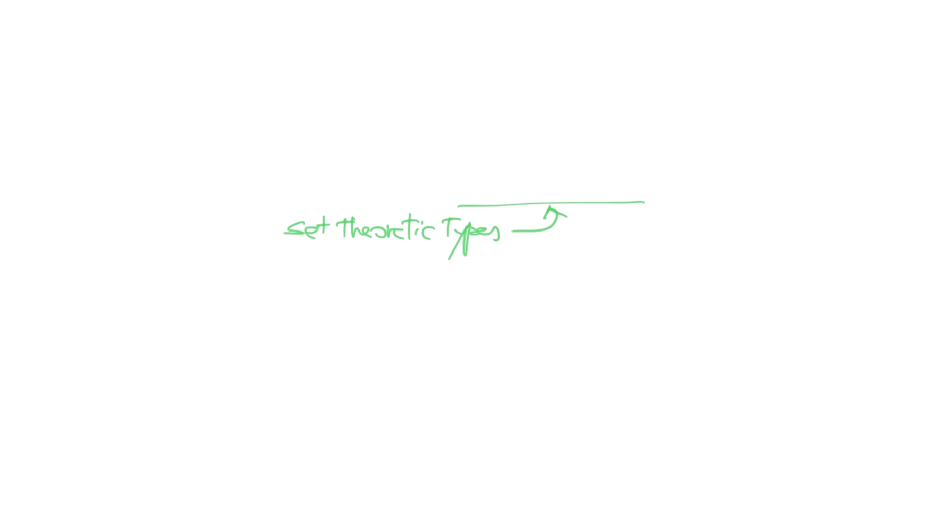
\includegraphics[scale=1]{images/hw-settheore.pdf}\end{textblock}}%
\only<3>{\begin{textblock}{5}(0,0)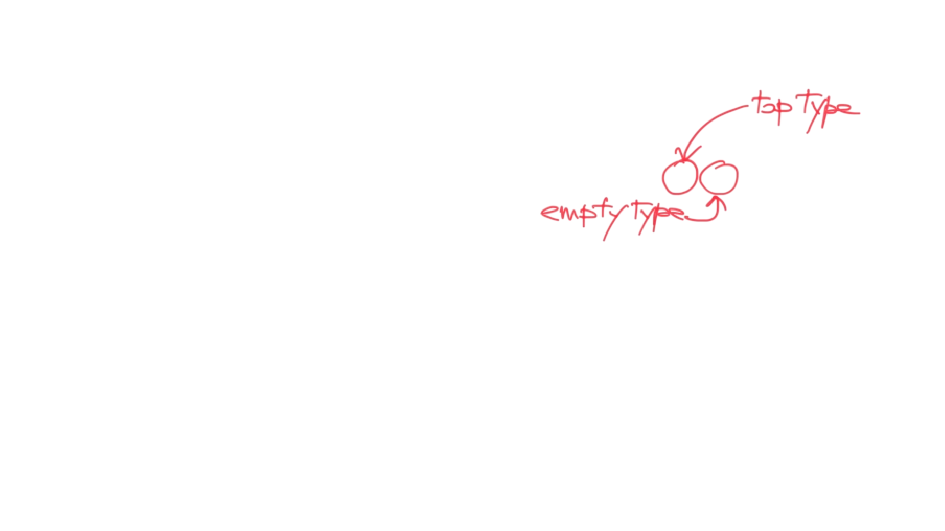
\includegraphics[scale=1]{images/hw-topbottom.pdf}\end{textblock}}%
\pause[4]%
\medskip
\textbf{\color{darkslateblue}The values that match a pattern $p$ form a type}:
\centerline{\color{magenta}
$\accept{p} = \{ v\mid v\text{ is a value that matches }p\}
$}

\textbf{\color{darkslateblue}(the accepted type of pattern $p$)}, e.g., $\Bl\accept{\patpair{x}{y}}=\pair\Any\Any$, the type of all pairs.
\end{frame}



\begin{frame}
\frametitle{3. Precise typing of pattern matching (II)}\xdef\matchframenumber{\insertframenumber}\transdissolve<4>% \matchframenumber is referenced in core.tex

\textbf{\color{darkslateblue}Boolean type connectives are needed to type pattern matching:}

\smallskip

    \hspace*{5mm}{\Bl$\texttt{ match }  e  \texttt{ with } p_1 \texttt{ -> } e_1 \texttt{ | } p_2\texttt{ -> } e_2$}

   \smallskip

Suppose that $\Bl e:\T$\vspace{2mm}
{\setlength{\leftmargini}{0.75em}\setlength{\labelsep}{0.3em}%
\begin{itemize}\setlength{\topsep}{3.5mm}\setlength{\itemsep}{0.2mm}
\item To infer the type $\Bl\T_1$ of $\Bl e_1$ we need {\color{blue}$\T\And \accept{p_1}$};
\item To infer the type $\Bl\T_2$ of $\Bl e_2$ we need {\color{blue}$(\T\setminus \accept{p_1})\And \accept{p_2}$;}\hfill{\textcolor{gray}{\small($\texttt{S}\setminus\T = \texttt{S}\!{\And}\!\neg{\T}$: negation)}}
\pause
\item The type of the match expression is {\color{blue}$\T_1\Or \T_2$}.
\item Pattern matching is exhaustive if $\color{blue}\T\leq\accept{p_1}\Or \accept{p_2}$.
\end{itemize}}
\vspace{-1mm}
\pause
\textbf{Formally:}
\vspace{-2mm}
\begin{mathpar}\Bl
\infer[{[Match]}]
{\Gamma\vdash e:\T\and\Gamma, \T\!\!\And\!\!\accept{p_1\!}/p_1\vdash e_1:\T_1\and \Gamma, \T\setminus\accept{p_1\!}/p_2\vdash e_2:\T_2}
{\Gamma\vdash \texttt{match } e \texttt{ with }p_1 \texttt{->} e_1 \texttt{ | }p_2 \texttt{->} e_2 : \T_1\Or\T_2 }\mbox{\small($\T\leq\accept{p_1\!}\Or\accept{\!p_2\!}$)}
\end{mathpar}
\vspace{-4mm}

\small\color{gray}
where $\Bl \T/p$ is the type for the capture variables in $\Bl p$ when it is matched against values in $\Bl \T$.

\only<4>{\begin{textblock}{5}(0,0)
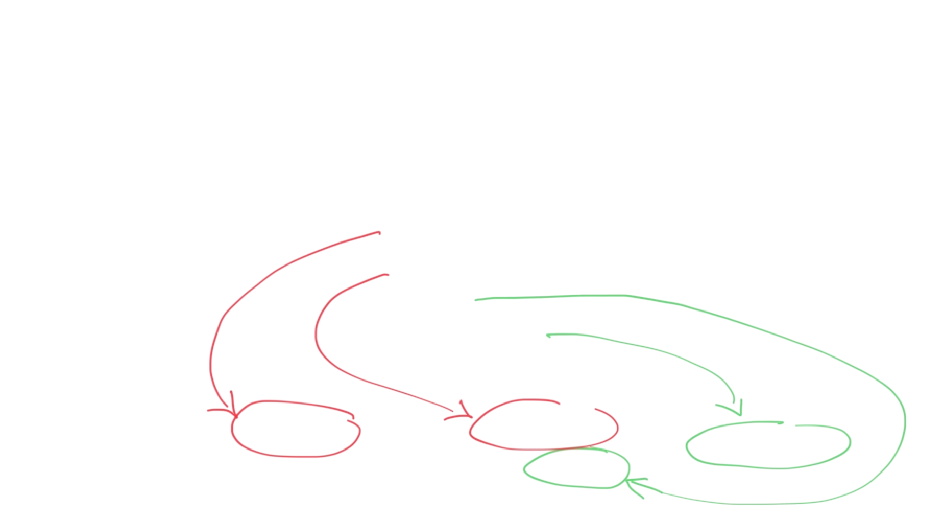
\includegraphics[scale=1]{images/hw-caseexp.pdf}
\end{textblock}}
\end{frame}

\subsection{Semantic subtyping}
\begin{frame}
\frametitle{Semantic subtyping}\vspace{-4mm}

Union and intersection types are now common (TypeScript, Python, Scala 3, Ceylon, \ldots);
negation types are rare.

\smallskip
\textbf{\color{darkslateblue}Our approach: \emph{semantic subtyping}, i.e., subtyping defined by what types mean.}

\smallskip
\begin{columns}[T,onlytextwidth]
  \begin{column}{0.58\textwidth}
    \begin{block}{How does it work?}
      \begin{enumerate}\setlength{\itemsep}{1pt}
        \item Types denote sets of values: $\sem{t}$
        \item Connectives are set operations:\\
              $\sem{t\vee s}=\sem{t}\cup\sem{s}\quad\sem{t\wedge s}=\sem{t}\cap\sem{s}$\\
              $\sem{\neg t}=\sem{t}^{\complement}$
        \item Subtyping is inclusion:\quad $t\leq s \iff \sem{t}\subseteq\sem{s}$
        \item Derive algorithms to decide $\leq$ and compute type operators
      \end{enumerate}
    \end{block}
  \end{column}
  \begin{column}{0.39\textwidth}
    \begin{block}{Why not subtyping rules?}
      Rule-based systems end up incomplete and fragile: e.g.,\\[1mm]
      \centerline{$(\Int\vee\Bool)\times\Int\ \leq$}
      \centerline{$(\Int\times\Int)\vee(\Bool\times\Int)$}\vspace{1mm}
      may not be derivable.

      \smallskip
      With semantic subtyping, all set-theoretic laws hold for \textbf{free}.
    \end{block}
  \end{column}
\end{columns}

\end{frame}
